\chapter{Colorful $k$-center}
\label{cap:colkcenter}
The first problem addressed is the colorful $k$-center. 
Its definition is recalled, and then a 3-approximation due to Jia, Sheth, and Svensson~\cite{JSS2020} is presented. This algorithm is referred to as the JSS approximation.

\begin{problem}[Colorful $k$-center]
Given a metric space $(P,d)$, where $P$ is a point set partitioned into $c$ color classes $\set{P_1,\ldots,P_c}$ and $d : P \times P \to \mathbb{R}_+$ is a metric, a vector of coverage requirements $t \in \mathbb{Z}^c$, and an integer $k$,
the goal of the \emph{colorful $k$-center} problem is to find a set $S \subseteq P$ of size at most $k$ and a set $C \subseteq P$ such that $|C \cap P_i| \geq t_i$ for each $i \in [c]$, and $S$ and $C$ minimize $\max_{j \in C} d(j,S)$.
\end{problem}

Equivalently, the goal is to find the smallest radius $\rho$ such that one can choose $k$ points in $P$ and place $k$ balls of radius $\rho$ around them to satisfy the coverage requirement for every color class. For a metric $(P,d)$ and for each $p \in P$ and $r \in \mathbb{R}_{\geq 0}$, the set $\mathcal{B}(p,r) \coloneqq \set{j \in P : d(j,p) \leq r}$ is the \emph{ball} of radius $r$ centered at $p$. For convenience, $\mathcal{B}(p) \coloneqq \mathcal{B}(p,1)$ is defined for each $p \in P$.


From now on, the attention is restricted to the two-color case, defining
\[
  R\coloneqq P_1,\quad
  B \coloneqq P_2,\quad
  \rho \coloneqq t_1 ,\quad
  \beta \coloneqq t_2,
\]
where $R$ denotes the set of red points and $B$ denotes the set of blue points.
Without loss of generality, it is assumed that the problem instances are normalized so that the optimal value is 1. 
This is justified by the observation that the optimal radius must belong to the set of $O(n^2)$ pairwise distances between points in $P$. 
By iterating over these $O(n^2)$ candidate distances and scaling the instance accordingly, it is guaranteed that at least one such instance satisfies this normalization.

A pseudo $\alpha$-approximation for the colorful $k$-center problem is a polynomial-time algorithm that, given an instance $(R,B,\rho,\beta,d,k)$, finds sets $S$ and $C$ of points such that $|S| \leq k + O(1)$, $|C \cap R| \geq \rho$, $|C\cap B| \geq \beta$, and $\max_{j\in C}d(j,S) \leq \alpha \,\OPT$, where $\OPT$ is the optimal value for the instance. That is, the algorithm finds a solution that satisfies the coverage constraints and has a bounded value compared to the optimal one, but relaxes the constraint on the number of open centers. First, a pseudo 2-approximation algorithm for the colorful \(k\)-center problem, due to Bandyapadhyay, Inamdar, Pai, and Varadarajan~\cite{BIPV2019} is presented, which will be used as a subroutine in the JSS approximation.

\subsection{Pseudo approximation for the colorful $k$-center}

The pseudo approximation presented here is due to Bandyapadhyay \emph{et al.}~\cite{BIPV2019}, but has a simple modification due to Jain \emph{et al.}~\cite{JSS2020}, which will be presented here.

Let \(I = (R,B,\rho,\beta,d,k)\) be a two-color instance of the colorful $k$-center problem with optimal value~1. 
The pseudo approximation presented here opens at most $k+1$ clusters with radius at most 2.
Set $P \coloneqq R \cup B$.
Now, consider the following linear program.

\begin{equation}\tag{LP1} \label{LP1}
\begin{aligned}
\sum_{i\in \cball(j)} \; x_i &\ge z_j,
  &&\forall\,j\in P,\\
\sum_{i\in P} x_i &\le k,\\
\sum_{j\in R} z_j &\ge \rho,\\
\sum_{j\in B} z_j &\ge \beta,\\
x,z &\in[0,1]^P.
\end{aligned}
\end{equation}

Here, the variable $x_i$ indicates how much the point $i$ is (fractionally) open as a center, while $z_i$ indicates how much the point $i$ is covered by centers in $\mathcal{B}(i)$. 
Note that the feasible solutions for this program represent fractionally open centers that fractionally cover points located within a unit radius, satisfying the coverage constraints. 
Since $I$ has optimal value 1, the program is feasible.

The pseudo approximation algorithm proceeds in two phases. 
In the first phase, \eqref{LP1} is solved to generate a set of candidate clusters; in the second phase, at most \(k+1\) clusters are selected from these candidates. 
For the algorithm of the first phase, the following definition is used.
\begin{definition}
    For each $j \in P$, the set $\mathcal{F}(j) \coloneqq \bigcup_{i \in \cball(j)}\cball(i)$ is the \emph{flower set} of $j$.
\end{definition}
\begin{figure}[h]
    \centering
    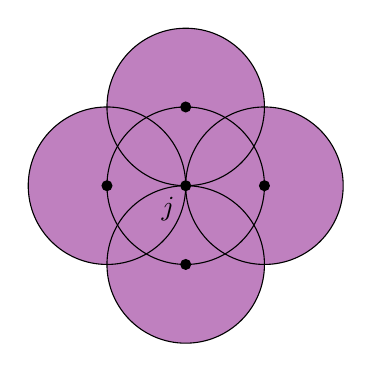
\begin{tikzpicture}

\coordinate (j) at (0,0);
\coordinate (A) at (0,1);
\coordinate (B) at (-1,0);
\coordinate (C) at (1,0);
\coordinate (D) at (0,-1);

\begin{scope}
  \fill[violet!50] (j) circle(1);
  \fill[violet!50] (A) circle(1);
  \fill[violet!50] (B) circle(1);
  \fill[violet!50] (C) circle(1);
  \fill[violet!50] (D) circle(1);
\end{scope}

\draw (j) circle(1);
\draw (A) circle(1);
\draw (B) circle(1);
\draw (C) circle(1);
\draw (D) circle(1);


\foreach \point in {j,A,B,C,D}
  \fill (\point) circle (2pt);

\node at (j) [below left=0.5pt] {$j$};
\end{tikzpicture}
    \caption{Points in $P$ within the purple region form the flower set of point $j$.}
\end{figure}

\subsubsection{Phase one}

The first phase is given by {\bf Algorithm~\ref{Alg1}}, which builds a set of candidate clusters. 
First, an optimal solution~$(x,z)$ of~\eqref{LP1} is taken. 
Then, a point with the highest $z$-value is iteratively taken from the remaining point set to be the center of a cluster, and the remaining points of its flower set compose its cluster. 
The point set is updated and the algorithm continues until no points with positive $z$-values remain. 
Moreover, vectors $y$ and $\tilde{z}$ are built which will help to prove the quality guarantee of the selected clusters, although they are not the final solution.

\begin{algorithm}
    \caption{\sc FindCandidates\((R,B,\rho,\beta,d,k)\)}
    \label{Alg1}
    \begin{algorithmic}[1]
        \State Let $(x,z)$ be a solution of~\eqref{LP1} for $R, B, k, \rho, \beta$ using $d$. 
        \State $S \gets \emptyset$, $\quad$ $P' \gets R \cup B$
        % If LP1 is infeasible, then the instance inserted has no fractional solution of value 1.
        \While{$P' \neq \emptyset$ and $\max_{j \in P'} z_j > 0$}
        \State Let $j \in \arg\max_{\ell \in P'} z_\ell$.
        \State $S \gets S \cup \set{j}$
        \State $y_j \gets \min\set{1,\sum_{i\in\cball(j)} x_i}$
        \State $\tilde{z}_j \gets y_j$
        \State $C_j \gets \mathcal{F}(j)\cap P'$
        \For{all $j' \in C_j\setminus\set{j}$}
        \State $y_{j'} \gets 0$, \quad $\tilde{z}_{j'} \gets \tilde{z}_j$
        \EndFor
        \State $P' \gets P' \setminus C_j$
        \EndWhile
        \State \Return $\Big(S,\left\{ C_j : \,j \in S \right\} \Big)$
    \end{algorithmic}
\end{algorithm}
It is clear that {Algorithm~\ref{Alg1}} runs in polynomial time, since solving a linear program can be done in polynomial time, and all the other steps of the algorithm also run in polynomial time.

The next two theorems prove that candidate clusters meet the color requirements and that the points of a cluster have the distance to the cluster center bounded by 2.
First, this distance is bounded for the points inside one candidate cluster.

\begin{theorem}
    \label{dist_upb}
    If $j \in S$ and $i \in C_j$, then $d(i,j) \leq 2$.
\end{theorem}
\begin{proof}
    
By definition of $C_j$, one has $i \in \mathcal{F}(j)$. Thus, there is \(h \in \cball(j)\) such that \(i \in \cball(h)\). Therefore,
\[
d(i,j)
\;\le\; d(i,h) + d(h,j)
\;\le\; 1 + 1 \;=\; 2,
\]
where the first inequality holds by the triangle inequality, and the last by the definition of $\cball(j)$ and $\cball(h)$.
\end{proof}

Now it is proved that the candidate clusters meet the coverage requirements. 
To this end, another linear program is introduced. 
For each $j \in S$, set 
\[
r_j \coloneqq |C_j \cap R|\text{ and } b_j \coloneqq |C_j \cap B|.
\] 
Then, consider the following linear program for vectors $r$ and $b$.

\begin{equation}\tag{LP2} \label{LP2}
\begin{aligned}
    \text{Maximize} \quad &\sum_{j \in S} r_j y_j\\
    \text{subject to} \quad& \sum_{j \in S} b_jy_j \geq \beta, \\
    &\sum_{j \in S} y_j \leq k,\\
    & y \in [0,1]^S.
\end{aligned}
\end{equation}
%
Set $\tilde{C} \coloneqq \bigcup_{j \in S} C_j$. 
Let $y$ be the vector produced by {Algorithm~\ref{Alg1}}. 
Note that \[
|\tilde{C} \cap R| = \sum_{j \in S} |C_j \cap R| = \sum_{j \in S} r_j \geq \sum_{j \in S} r_j y_j,
\]
and 
\[
|\tilde{C} \cap B| = \sum_{j \in S} |C_j \cap B| = \sum_{j \in S} b_j \geq \sum_{j \in S} b_j y_j.
\]
Therefore, if $y$ is a feasible solution of~\eqref{LP2} with objective value at least $\rho$, then the candidate clusters satisfy the coverage requirements.

\begin{theorem}
    \label{feas:LP2}
The vector $y$ produced by \textrm{\bf Algorithm~\ref{Alg1}} is a feasible solution of~\eqref{LP2} with objective value at least $\rho$.    
\end{theorem}

\begin{proof}
    First, note that, for each $i \in P$, there is at most one $j \in S$ with $d(i,j) \leq 1$, that is, the unit balls centered at points in $S$ do not overlap.
    Indeed, assume, for the sake of contradiction, that there are $j,j' \in S$ such that $j,j' \in \mathcal{B}(i)$ and that $j$ was added to $S$ before $j'$. Then, $j' \in C_j$ and $j'$ would have been removed from $P'$ and, could not be chosen to be part of $S$ after that, a contradiction.
    Now, observe that, for each $i \in \tilde{C}$ with $i \in C_j$ for some $j \in S$, one has ${\tilde{z}_j = \tilde{z}_i \geq z_i}$. It is evident that this holds if $\tilde{z}_j = 1$, otherwise  
    \begin{equation}
        \label{z-bound}
    \tilde{z}_j = \sum_{h \in \cball(j)} x_h \geq z_j \geq z_i, 
    \end{equation}
    where the first inequality holds because of the first constraint of~\eqref{LP1} and the second inequality holds because $i$ was in $P'$ when $j$ was chosen to join $S$ and by the choice of~$j$ in line 4 of~{Algorithm~\ref{Alg1}}.

    Now, let us argue that $y$ is feasible for~\eqref{LP2} with objective value at least $\rho$. For each $j \in S$, set $R_j \coloneqq C_j \cap R$. Note that 
    \begin{align*}
        \sum_{j \in S} r_jy_j &= \sum_{j \in S} r_j \tilde{z}_j = \sum_{j \in S} \sum_{i \in R_j} \tilde{z}_j
        \geq \sum_{j \in S} \sum_{i \in R_j} z_i \,\,= \! \sum_{i \in R: z_i > 0 } z_i = \sum_{i \in R} z_i \geq \rho,
    \end{align*}
    where the first equality holds by the definition of $\tilde{z}$, the second equality holds by the definition of $r_j$, the first inequality holds by~\eqref{z-bound}, the third equality holds because, by construction, the $C_j$'s are disjoint and contain all points with positive $z$-values, and the last inequality holds by the third constraint of~\eqref{LP1}. Similarly, \(\sum_{j \in S } b_jy_j \geq \beta\). Now, we must prove that \(\sum_{j \in S} y_j \leq k\). Note that
    \begin{align*}
    \sum_{j \in S} y_j \leq \sum_{j \in S} \sum_{i \in \cball(j)}x_i \leq \sum_{i \in P} x_i \leq k,
    \end{align*}
    where the first inequality holds by the definition of $y$, the second holds from the claim that the unit balls centered at points in $S$ are disjoint, and the last one holds because $x$ satisfies the second constraint of~\eqref{LP1}.
\end{proof}

The pseudo approximation is completed by using~\eqref{LP2} to choose, in phase two, some clusters from the candidates.

\subsubsection{Phase two}

The second phase begins by utilizing the candidate clusters from phase one to define the constraints of~\eqref{LP2}. 
From an extreme-point optimal solution of this program, the set of clusters corresponding to positive $y$-values is extracted, which constitutes the pseudo solution. The steps of this construction are summarized in the algorithm below. Here, the acronym BIPV is used to refer to the method proposed by Bandyapadhyay, Inamdar, Pai, and Varadarajan~\cite{BIPV2019}.

\begin{algorithm}
    \caption{\sc BIPV\((R,B,\rho,\beta,d,k)\)}
    \label{Alg2}
    \begin{algorithmic}[1]
        \State $\left(S,C\right) \gets \text{\sc FindCandidates}(R,B,\rho,\beta,d,k)$
        \For{$j \in S$}
        \State $r_j \gets |R \cap C_j|$
        \State $b_j \gets |B \cap C_j|$
        \EndFor
        \State Let $y^*$ be an extreme-point optimal solution of~\eqref{LP2} for $S$ and vectors $r$ and $b$.
        \State $S^* \gets \set{i \in S : y_i^* > 0}$
        \State \Return $\left(S^*,\bigcup_{j\in S^*}C_j\right)$
    \end{algorithmic}
\end{algorithm}
It is clear that this algorithm runs in polynomial time, since finding an extreme‐point optimal solution to a linear program can be done in polynomial time.
Let $\left(S^*,C^*\right)$ be the solution returned by {Algorithm~\ref{Alg2}}. 
By Theorem~\ref{dist_upb}, for each $i \in C^*$, one has ${d(i,S^*) \leq d(i,j) \leq 2}$, where $j \in S^*$ is such that $i \in C_j^*$. 
Moreover, the coverage requirements are satisfied. 
The blue requirement follows from the first constraint of~\eqref{LP2}, and the red requirement holds because Theorem~\ref{feas:LP2} shows that there is a solution of~\eqref{LP2} with objective value at least $\rho$. It remains to bound the size of $S^*$.

\begin{theorem}
    \label{size_upb}
    Let $\left(S^*,C^*\right)$ be the solution returned by {Algorithm~\ref{Alg2}}. Then, \[|S^*| \leq k+1.\]
\end{theorem}
%
\begin{proof}
    Since~\eqref{LP2} has exactly two non-trivial constraints, every extreme-point solution has at most two strictly fractional variables. This is a classic result from linear algebra which is implied by Lemma 2.1.4 in~\cite{LauRaviSingh2011}. If it has at most one strictly fractional variable, then the statement trivially holds. Thus, suppose that there are $i,i' \in S^*$ which have strictly fractional $y^*$-values. Then, one has
    \[k \geq \sum_{j \in S^*} y^*_j  = y_{i}^* + y_{i'}^* + \sum_{j \in S^* \setminus \set{i,i'}} y^*_j = y_{i}^* + y_{i'}^* + |S^*| - 2\]
    and thus $|S^*| \leq k + (2 - y_{i}^* - y_{i'}^*) < k + 2$. Since $|S^*|$ and $k$ are integers, one can deduce that $|S^*| \leq k +1$.
\end{proof}

Finally, the following theorem that summarizes the discussed pseudo approximation is stated.

\begin{theorem}
    \label{pseudo_guarantee}
    Let $ I = (R,B,\rho,\beta,d,k)$ be a two-color instance for the $k$-center problem with optimal value 1. There exists a polynomial-time algorithm that finds $S \subseteq R \cup B$ and $C \subseteq R\cup B$ such that
    \begin{enumerate}
        \item $|S| \leq k+1$;
        \item for each $j \in C$, there is an $i \in S$ such that $d(i,j) \leq 2$;
        \item $|C \cap R| \geq \rho$;
        \item $|C \cap B| \geq \beta$.
    \end{enumerate}
    This polynomial-time algorithm is a pseudo $2$-approximation for the $k$-center problem.
\end{theorem}

\subsection{3-Approximation for the colorful $k$-center}
Now the JSS approximation is presented. 
Here the focus is on the two color version, but you can find a generalization for any constant number of colors in Section 3 of~\cite{JSS2020}.

Let $I = (R,B,\rho,\beta,d,k)$ be a two-color instance of the colorful $k$-center problem with optimal value 1. 
Using the approach employed in the pseudo approximation, one can find $k$ clusters of radius 2 that cover at least $\beta$ blue points and at least $\rho - \max_{j \in S} r_j$ red points, where $S$ is the set of $k$ cluster centers and $r_j$ is the number of red points in the cluster centered at $j$. 
The only difference from the pseudo approximation approach is that, instead of selecting all clusters with positive $y^*$-values in line 6 of {Algorithm}~\ref{Alg2}, only those with $y_j^*=1$ are selected, and the one with fractional $y^*$-value that covers the greatest number of blue points. 
This result is formalized in the following lemma.
\begin{lemma}[Lemma 1 in~\cite{JSS2020}]
    \label{pseudo_to_approx}
    Let $(R,B,\rho,\beta,d,k)$ be a two-color instance for the colorful $k$-center problem with optimal value 1. There exists a polynomial-time algorithm that finds a set $S \subseteq R \cup B$ such that 
    \begin{enumerate}
        \item \( |S| \leq k\);
        \item 
        \(
            \Big| \bigcup_{j \in S} \mathcal{F}(j) \cap B\Big| \geq \beta
            \);
        \item
        \(
            \Big| \bigcup_{j \in S} \mathcal{F}(j) \cap R\Big| \geq \rho - \max_{j \in S} | \mathcal{F}(j) \cap R|.
        \)
    \end{enumerate}
\end{lemma}
This approach, by itself, is insufficient to yield an approximation algorithm for the problem. 
However, it will be a key point of the JSS approximation. 
The core intuition of what follows is that, if the number of red points in each cluster is small, the red points deficit incurred in item~3 of Lemma~\ref{pseudo_to_approx} can be compensated by slightly expanding the clusters radius.

With the goal of eventually bounding the number of red points in each cluster, the instances of the colorful $k$-center problem are first partitioned into two types, according to the following definition.

\begin{definition}
    Let $I = (R,B,\rho,\beta,d,k)$ be a two-color instance of the colorful $k$-center problem with optimal value $1$.
    We say that $I$ is \emph{well-separated} if no ball of radius 3 centered at a point in $R \cup B$ covers at least two unit balls with centers at some optimal solution center of $I$.
\end{definition}

First a 3-approximation for non-well-separated instances is presented, which uses {Algorithm~\ref{Alg2}} as a subroutine. Note that it is not known whether the given instance is well-separated or not, or which specific point $j \in R \cup B$ has a ball $\mathcal{B}(j, 3)$ containing at least two unit balls centered at points of some optimal solution. Thus, the algorithm guesses this point by trying every possible $j \in R \cup B$. For each guess, the instance is updated by removing the points covered by $\mathcal{B}(j, 3)$ and reducing the number of centers to open by 2. Then, {Algorithm~\ref{Alg2}} (BIPV) is run on the residual instance. If the instance is not well-separated, in the correct guess, ~\eqref{LP1} will be feasible and the algorithm will return a valid solution with one ball of radius 3. Note that BIPV does not solve the linear program~\eqref{LP1} directly; instead, it calls {Algorithm~\ref{Alg1}}, which computes its solution.

\begin{algorithm}[H]
\caption{Non-well-separated-instances($R, B, \rho, \beta, d, k$)}
    \label{non-separated-algo}
    \begin{algorithmic}[1]
    \For{each $j \in R \cup B$}
        \State $R_j \gets R \cap \mathcal{B}(j, 3)$
        \State $B_j \gets B \cap \mathcal{B}(j, 3)$
        \If{\eqref{LP1} is feasible for $R \setminus R_j, B \setminus B_j, \rho - |R_j|, \beta - |B_j|, d, k - 2$}
            \State $(S,C) \gets$ BIPV($R \setminus R_j, B \setminus B_j, \rho - |R_j|, \beta - |B_j|, d, k - 2$)
            \State \Return $(S \cup \{j\}, C \cup \mathcal{B}(j, 3))$
        \EndIf
    \EndFor
    \end{algorithmic}
\end{algorithm}

It is easy to see that {Algorithm~\ref{non-separated-algo}} is indeed a 3-approximation for instances that are not well-separated. It produces a very particular solution, because it uses only one cluster of radius 3 and all the other clusters have radius 2.
\begin{theorem}
    \label{non-separated-theorem}
    {\rm {Algorithm~\ref{non-separated-algo}}} is a 3-approximation for non-well-separated instances.
\end{theorem}
\begin{proof}
Let $I = (R, B, \rho, \beta, d, k)$ be a non-well-separated instance with optimal value 1. Because the instance is non-well-separated, there exists at least one point $j^* \in R \cup B$ such that $\mathcal{B}(j^*, 3)$ contains at least two unit balls centered at points of some optimal solution OPT for $I$. 
The algorithm iterates over all points in $R \cup B$. Consider the iteration where $j = j^*$. At this point, $R_{j^*} := R \cap \mathcal{B}(j^*, 3)$ and $B_{j^*} := B \cap \mathcal{B}(j^*, 3)$ are defined. Because $\mathcal{B}(j^*, 3)$ covers at least two unit balls centered at points of $\OPT$, the remaining set $\text{OPT} \setminus \mathcal{B}(j^*, 3)$ has size at most $k - 2$ and the unit balls centered at them cover at least $\rho - |R_{j^*}|$ red points and $\beta - |B_{j^*}|$ blue points from $R \setminus R_{j^*}$ and $B \setminus B_{j^*}$.
Therefore, the optimal value of the instance $(R \setminus R_{j^*}, B \setminus B_{j^*}, \rho - |R_{j^*}|, \beta - |B_{j^*}|, d, k - 2)$ is also bounded by 1, which implies that~\eqref{LP1} on them is feasible. As guaranteed by Theorem~\ref{pseudo_guarantee}, the BIPV algorithm will successfully return a pseudo solution $(S, C)$.
Thus, the algorithm is guaranteed to return a solution $(S', C')$ at some iteration (either at $j = j^*$ or earlier). Let $(S, C)$ be the solution returned by BIPV in that iteration. Setting $S' := S \cup \{j\}$ and $C' := C \cup \mathcal{B}(j, 3)$, one has by Theorem~\ref{pseudo_guarantee}:
\begin{enumerate}
    \item $|S'| = |S \cup \{j\}| = |S| + 1 \le (k - 2 + 1) + 1 = k$;
    \item $|C' \cap B| = |C \cap B| + |B_j| \ge \beta - |B_j| + |B_j| = \beta$;
    \item $|C' \cap R| = |C \cap R| + |R_j| \ge \rho - |R_j| + |R_j| = \rho$.
\end{enumerate}
Also, it is easy to see that, for each $c \in C'$, there is an $i \in S'$ such that $d(i, c) \le 3$. Since iterating over $O(n)$ points preserves the polynomial running time, {Algorithm~\ref{non-separated-algo}} is a 3-approximation for non-well-separated instances.
\end{proof}

Next, we present a 2-approximation for well-separated instances.
The algorithm proceeds in two phases. 


\subsubsection{Phase one}

Let $(R, B, \rho, \beta, d, k)$ be a well-separated instance with optimal value 1, and let $\OPT$ be the set of cluster centers of an optimal solution for this instance. 
In this phase, the instance is preprocessed with two objectives:
\begin{enumerate}
    \item to ensure that certain clusters contain a sufficient number of red points;
    \item to bound the number of red points in any future cluster.
\end{enumerate}
These two objectives pave the way for the application of Lemma~\ref{pseudo_to_approx} later in the analysis.
The preprocessing step consists of finding three clusters of radius 2 that each contain a unit ball centered at a point of $\OPT$ that maximizes the number of red points that are in the cluster, but not in the unit ball.  
Subsequently, the point set is updated by removing those clusters.

First, the notion of $\mathrm{Gain}(p,q)$ is defined for any point $p \in P$ and $q \in \mathcal{B}(p)$. See Figure~\ref{Fig2}.

\begin{definition}
    Let $p \in P$ and $q \in \mathcal{B}(p)$. Set $\mathrm{Gain}(p,q) \coloneqq R \cap \left(\mathcal{F}(q) \setminus \mathcal{B}(p)\right)$.
\end{definition}

\begin{figure}[h]
    \centering
    \begin{tikzpicture}

\coordinate (q) at (0,0);
\coordinate (p) at (0,1);
\coordinate (B) at (-1,0);
\coordinate (C) at (1,0);
\coordinate (D) at (0,-1);

\begin{scope}
  \fill[red!50] (q) circle(1);
  \fill[red!50] (B) circle(1);
  \fill[red!50] (C) circle(1);
  \fill[red!50] (D) circle(1);
  \fill[white] (p) circle(1);
\end{scope}

\draw (j) circle(1);
\draw (A) circle(1);
\draw (B) circle(1);
\draw (C) circle(1);
\draw (D) circle(1);


\foreach \point in {j,A,B,C,D}
  \fill (\point) circle (2pt);

\node at (q) [below left=0.5pt] {$q$};
\node at (p) [below left=0.5pt] {$p$};
\end{tikzpicture}
    \caption{Red points in the red region form the gain set of the pair $(p,q)$.}
    \label{Fig2}
\end{figure}

Using this definition, the instance is updated three times by guessing points $c$ of $\OPT$ which maximize the size of Gain$(c,q)$ for some $q \in \mathcal{B}(c)$.
Set $P_1\coloneqq P$.
First, try all tuples $(c_1, c_2, c_3)$ and, for $i = 1, 2, 3$, sequentially select $q_i \in \mathcal{B}(c_i)$ so that the number of (red) points in $Gain(c_i, q_i) \cap P_i$ is maximized, where
        \( P_i = P_{i-1} \setminus \mathcal{F}(q_{i-1}) \text{ for } 2 \le i \le 4. \)
It takes time $O(n^3)$ to guess all tuples and, for each $c_i$, it takes time $O(n)$ to find a $q_i \in \mathcal{B}(c_i)$ as above. 
Set $\mathrm{Guess} \coloneqq \bigcup_{i =1}^3 \mathcal{B}(c_i)$ and let $\tau \coloneqq |\mathrm{Gain}(c_3,q_3) \cap P_3|$. 
The reason that three points are guessed is because, later, up to $3\tau$ red points will be lost after closing a center opened by running the pseudo approximation on a preprocessed instance. 
After updating the instance three times, the following lemma states what is guaranteed in the new instance.

\begin{lemma}[Lemma 2 in~\cite{JSS2020}]
    \label{lemma: c's}
    Assuming that $c_1,c_2$ and $c_3$ are guessed correctly, we have that
    \begin{enumerate}
        \item the $k-3$ unit balls centered at points in $\OPT\setminus\{c_i\}_{i=1}^3$ cover ${\beta - |B \cap \mathrm{Guess}|}$ blues points and ${\rho - |R \cap \mathrm{Guess}|}$ red points of $P_4$; and
        \item the three clusters $\mathcal{F}(q_1), \mathcal{F}(q_2)$ and $\mathcal{F}(q_3)$ are contained in $P \setminus P_4$ and cover at least  $|B \cap \mathrm{Guess}|$ blue points and at least $|R \cap \mathrm{Guess}| + 3 \tau$ red points.
    \end{enumerate}
\end{lemma}

\subsubsection{Phase two}
Let $(R, B, \rho, \beta, d, k)$ be a well-separated instance with optimal value 1, and let $\OPT$ be the set of cluster centers of an optimal solution for this instance.  
It is initially assumed that $c_1, c_2,$ and $c_3$ have been correctly guessed such that Lemma~\ref{lemma: c's} holds. 
Furthermore, it is assumed that we have the new point set $P_4$, the value $\tau$, and the set $\mathrm{Guess}$ as established in the previous phase.

Note that, by the $\tau$ definition, for any $p \in P_4 \cap \OPT$ and $q \in \mathcal{B}(p) \cap P_4$, one has 
\begin{equation}
    \label{eq:tau}
|\mathrm{Gain}(p,q) \cap P_4| \leq \tau.
\end{equation}
This holds especially for $p=q$ and implies that $\mathcal{F}(p)\setminus\mathcal{B}(p)$ contains at most $\tau$ red points of $P_4$. To compensate the $\max_{j \in S} |\mathcal{F}(j) \cap R \cap P_4|$ red points lost in item 3 of Lemma~\ref{pseudo_to_approx}, we need to bound the number of red points in the flower set of any $j \in S$. Thus, the instance is divided into two instances using the following definition.

\begin{definition}
    For a set $P_s \subseteq P_4$, we say that $j \in P_s$ is \emph{dense} if the ball $\mathcal{B}(j)$ contains strictly more than $2\tau$ red points of $P_s$. For a dense point $j$, we also set ${I_j \coloneqq \{ i \in P_s : |\mathcal{B}(j) \cap \mathcal{B}(i) \cap R \cap P_s| > \tau \}}$, i.e., the set of $i \in P_s$ such that the intersection of the unit balls around $i$ and $j$ has strictly more than $\tau$ red points in $P_s$. Moreover, we say that $P_s$ is \emph{sparse} if it has no dense points.
\end{definition}

The idea here is to divide the set $P_4$ in a sparse set $P_s$ and a dense set $P_d$. For any $p \in P_s \cap \OPT$, one has
\begin{equation}
    \label{bound_red_flower_opt}
|\mathcal{F}(p) \cap R \cap P_s| = |(\mathcal{F}(p) \setminus \mathcal{B}(p) ) \cap R \cap P_s | + |\mathcal{B}(p) \cap R \cap P_s| \leq \tau + 2\tau = 3\tau,
\end{equation}
where $|(\mathcal{F}(p) \setminus \mathcal{B}(p) ) \cap R \cap P_s | \leq |\mathrm{Gain}(p,p) \cap P_s| \leq \tau$ by~\eqref{eq:tau}.
This just holds for points that are in OPT, and we do not have them. 
But it will be shown that, for $P_s$, some constraints can be added in~\eqref{LP1} so that, for each candidate cluster center $j$, it holds that $|\mathcal{F}(j) \cap R \cap P_s| \leq 3\tau$.

To construct the sparse set $P_s \subseteq P_4$, an iterative removal process is employed. 
Initially, let $P_s = P_4$ and $I = \emptyset$. 
While there exists a dense point $j \in P_s$, the set to be removed $D_j \coloneqq \bigcup_{i \in I_j} \mathcal{B}(i) \cap P_s$ is defined. 
Then, $P_s$ is updated by removing $D_j$, and the set $I_j$ is added to the set family $I$. 
This procedure results in a set $P_s$ with no dense points; then $P_s$ and its complement, $P_d \coloneqq P_4 \setminus P_s$, are clustered separately. 
The collection $I$ of the sets $I_j$ will be important to explain why the sets can be clustered separately and will also be used in the algorithm that clusters the points of $P_d$.

A lemma is now stated showing that the unit balls with centers at $\OPT \setminus \{c_i\}_{i=1}^3$ either cover points in $P_s$ or in $P_d$, but not points from both sets. Intuitively, this means that if a point of $\mathcal{B}(c)$, for $c \in \OPT \setminus \{c_i\}_{i=1}^3$, is removed from $P_s$ and added to $P_d$, the entire ball $\mathcal{B}(c)$ is transferred as well.

\begin{lemma}[Lemma 3 in~\cite{JSS2020}]
    \label{dense_sparse_dont_overlap}
    On the iterative removal process, let $P_s$ be the set of remaining points at the iteration in which a dense point $j$ is processed. Then, for any $c \in P_s \cap \OPT$, either $c \in I_j$ or $\mathcal{B}(c) \cap D_j = \emptyset$.
\end{lemma}
\begin{proof}
Let $c \in \OPT \setminus \{c_i\}_{i=1}^3$ and $I_j \in I$. 
Suppose $c \not \in I_j$. 
If $\mathcal{B}(c) \cap D_j \neq \emptyset$, then there exists a point in $\mathcal{B}(c) \cap \mathcal{B}(i) \cap P_s$ for some $i \in I_j$. 
Suppose that $i=j$, that is, $\mathcal{B}(c) \cap \mathcal{B}(j) \cap P_s \neq \emptyset$. Note that, since $c \in P_s$, $\mathcal{B}(c) \cap \mathcal{B}(j)$ has at most $\tau$ red points of $D_j$, otherwise $c$ would be in $I_j$. Thus, one has
\[
|(\mathcal{B}(j) \setminus \mathcal{B}(c)) \cap D_j \cap R| = |\mathcal{B}(j) \cap D_j \cap R| - |\mathcal{B}(j) \cap \mathcal{B}(c) \cap D_j \cap R| > 2 \tau - \tau = \tau,
\]
where the inequality holds because $j$ is dense and by the observation about the size of the set $\mathcal{B}(j) \cap \mathcal{B}(c) \cap D_j \cap R$ above. Thus, we have that 
\[\tau < |(\mathcal{B}(j) \setminus \mathcal{B}(c)) \cap D_j \cap R| \leq |\mathrm{Gain}(c,j) \cap P_4| \leq \tau,\]
a contradiction. Now, suppose that there is a point $p \in \mathcal{B}(c) \cap \mathcal{B}(i) \cap P_s$ for some $i \in I_j\setminus \set{j}$. Then, by the definition of $I_j$, one has ${|\mathcal{B}(i) \cap \mathcal{B}(j) \cap D_j \cap R| > \tau}$. Thus
\[\tau < |\mathcal{B}(i) \cap \mathcal{B}(j) \cap D_j\cap R| \leq |\mathrm{Gain}(c,p) \cap P_4| \leq \tau, \]
where the second equality holds because $\mathcal{B}(i) \subseteq \mathcal{F}(p)$ and $ \mathcal{B}(i) \cap \mathcal{B}(j) \cap \mathcal{B}(c) = \emptyset$, also a contradiction.
\end{proof}
The JSS approximation proceeds by guessing the size $k_d$ of the set $\OPT \cap P_d$, along with the numbers $\rho_d$ and $\beta_d$ of red and blue points of $P_d$ covered by the unit balls centered at these points.
Note that, by Lemma~\ref{lemma: c's}, there are $k_s \coloneqq k - 3 - k_d$ points in $\OPT \cap P_s$ and the unit balls centered at these points cover at least $\rho_s \coloneqq \rho - |R \cap \mathrm{Guess}| - \rho_d$ red and $\beta_s \coloneqq \beta - |B \cap \mathrm{Guess}| - \beta_d$ blue points of $P_s$. 
By Lemma~\ref{dense_sparse_dont_overlap}, the balls centered at points of $\OPT \cap P_s$ and points of $\OPT \cap P_d$ do not overlap.
There are $O(n^3)$ possible values of $k_d,\rho_d,\beta_d$ and all possibilities can be tried by increasing the running time by a factor of $O(n^3)$. 
Assuming that those parameters are correctly guessed, it is shown that the points of $P_d$ can be clustered in $k_d$ balls of radius one covering $\rho_d$ red points and $\beta_d$ blue points, and that the points of $P_s$ can be clustered in $k_s$ balls of radius two covering $\beta_s$ blue points and $\rho_s - 3\tau$ red points.

\begin{lemma}[Lemma 4 in~\cite{JSS2020}]
    \label{sparse_algo}
    There is a polynomial-time algorithm $\mathcal{A}_s$ that finds $k_s$ balls with radius two covering $\beta_s$ blue points and at least $\rho_s - 3\tau$ red points of $P_s$. 
\end{lemma}
\begin{proof}
The algorithm $\mathcal{A}_s$ is now described. By the assumption, there exist $k_s$ unit balls centered at points in $\mathrm{OPT} \cap P_s$ that cover $\beta_s$ blue points and $\rho_s$ red points of $P_s$. Hence, \eqref{LP1} has a feasible solution $(x,z)$ for the instance defined by the point set $P_s$, the number of clusters $k_s$, and the covering requirements $\beta_s$ and $\rho_s$.

By Lemma~\ref{pseudo_to_approx}, there is a polynomial-time algorithm that finds $S \subseteq P_s$ such that $|S| = k_s$ and the flowers centered at points of $S$ cover at least $\beta_s$ blue points and at least $\rho_s - \max_{j \in S} |\mathcal{F}(j) \cap R \cap P_s|$ red points. 

Suppose there is $j \in P_s$ such that $|\mathcal{F}(j) \cap R \cap P_s| > 3\tau$. If the constraint $x_i = 0$ is added for each $i \in \mathcal{B}(j) \cap P_s$, then $0 = \sum_{i \in \mathcal{B}(j) \cap P_s} x_i \geq z_j$. Thus, one must have $z_j = 0$. Since {Algorithm~\ref{Alg1}} only chooses points with positive $z$-values as candidate cluster centers, it follows that $|\mathcal{F}(j) \cap R \cap P_s| \leq 3\tau$ for each $j \in S$.

Let us argue that adding these constraints does not make \eqref{LP1} infeasible. Indeed, the integral solution representing the clusters centered at $\mathrm{OPT} \cap P_s$ remains feasible. This is proved by arguing that, for each $j \in P_s$ such that $|\mathcal{F}(j) \cap R \cap P_s| > 3\tau$, there is no $p \in \mathrm{OPT} \cap P_s$ such that $j \in \mathcal{B}(p)$, which implies $z_j = 0$.
Suppose, for the sake of contradiction, that there exists $p \in \mathrm{OPT} \cap P_s$ such that $j \in \mathcal{B}(p)$. Note that
\begin{align*}
    3\tau < |\mathcal{F}(j) \cap R \cap P_s| = |\mathrm{Gain}(p,j) \cap P_s| + |\mathcal{B}(p) \cap R \cap P_s| \leq |\mathrm{Gain}(p,j) \cap P_4| + 2\tau,
\end{align*}
where the first inequality holds by the choice of $j$, the equality holds by the definition of $\mathrm{Gain}(p,j)$, and the final inequality holds because $p$ is not a dense point. Thus, one has $\tau < |\mathrm{Gain}(p,j) \cap P_4| \leq \tau$ by~\eqref{eq:tau}, a contradiction. Consequently, there is no point of $\mathrm{OPT} \cap P_s$ in $\mathcal{B}(j)$, ensuring $z_j = 0$. Thus, it holds that $\max_{j \in S} |\mathcal{F}(j) \cap R \cap P_s| \leq 3\tau$, and Lemma~\ref{sparse_algo} is proved.
\end{proof}
\begin{lemma}[Lemma 4 in~\cite{JSS2020}]
    \label{dense_algo}
    There is a polynomial-time algorithm $\mathcal{A}_d$ that finds $k_d$ unit balls covering $\beta_d$ blue points and $\rho_d$ red points of $P_d$.
\end{lemma}
\begin{proof}
Now, the algorithm $\mathcal{A}_d$ is described.
By Lemma~\ref{dense_sparse_dont_overlap}, note that all $k_d$ unit balls centered at points in $\OPT \setminus \{c_i\}_{i=1}^3$ that cover points in $P_d$ are centered at points in $\bigcup_{I_j \in I} I_j$. Furthermore, one has that each $I_j$ contains at most one center of $\OPT$. This holds because $\mathcal{B}(i) \cap \mathcal{B}(j) \neq \emptyset$ for every $i \in I_j$. Thus, by the triangle inequality, $\mathcal{B}(j, 3)$ contains all balls $\{\mathcal{B}(i)\}_{i \in I_j}$. Hence, by the assumption that the instance is well-separated, the set $I_j$ contains at most one center of $\OPT$.

The problem is now reduced to a 3-dimensional subset-sum problem. For each $I_j \in I$, a group is formed consisting of an item for each $p \in I_j$. The item corresponding to $p \in I_j$ is the 3-dimensional value vector
$$(1, |\mathcal{B}(p) \cap D_j \cap B|, |\mathcal{B}(p) \cap D_j \cap R|).$$
The goal is to find $k_d$ items such that at most one item per group is selected, and their 3-dimensional vectors sum up to $(k_d, \beta_d, \rho_d)$. Such a solution, if it exists, can be found via standard dynamic programming utilizing a table of size $O(n^4)$. Furthermore, since the sets $D_j$ are disjoint by definition, this yields $k_d$ centers that cover $\beta_d$ blue points and $\rho_d$ red points in $P_d$, satisfying the statement of the lemma.

It remains to show that such a solution exists. Set $\{o_1, o_2, \ldots, o_{k_d}\} \coloneqq \OPT \cap P_d$. Furthermore, let $I_{j_1}, \ldots, I_{j_{k_d}}$ be the sets in $I$ such that $o_i \in I_{j_i}$ for $i \in \{1, \ldots, k_d\}$. Note that, by Lemma~\ref{dense_sparse_dont_overlap}, $\mathcal{B}(o_i)$ is disjoint from $P_d \setminus D_{j_i}$; that is, $\mathcal{B}(o_i) \subseteq D_{j_i}$. Thus, one has that the 3-dimensional vector corresponding to each $\OPT$ center $o_i$ equals
$$(1, |\mathcal{B}(o_i) \cap D_{j_i} \cap B|, |\mathcal{B}(o_i) \cap D_{j_i} \cap R|),$$
which is equivalent to simply $(1, |\mathcal{B}(o_i) \cap B|, |\mathcal{B}(o_i) \cap R|)$. Thus, the definition of the value vectors gives the correct contribution of points. Therefore, relying on the assumption that our guesses of $k_d$, $\beta_d$, and $\rho_d$ were correct, the sum of these vectors corresponding to $o_1, \ldots, o_{k_d}$ results precisely in the vector $(k_d, \beta_d, \rho_d)$. Thus, $k_d$ unit balls covering $\beta_d$ blue points and $\rho_d$ red points of $P_d$ can be found.
\end{proof}
With both lemmas established, the main theorem can be proved.

\begin{theorem}[Theorem 2 in~\cite{JSS2020}]
    There is a 2-approximation algorithm for well-separated instances of the $k$-center problem.
\end{theorem}

\begin{proof}
The JSS approximation starts by guessing the optimal radius and normalizing the instance. In phase one, it guesses the centers $c_1, c_2, c_3$. In Phase two, it guesses $k_d, \rho_d, \beta_d$. There are $O(n^2)$ choices for the optimal radius, $n$ choices for each $c_i$, and $n+1$ choices for each of $k_d, \rho_d, \beta_d$. Since all other steps of the algorithm run in polynomial time, the total running time is polynomial. The algorithm tries all these guesses and outputs the best solution found among all choices.

For the correct guesses, a solution with $3 + k_d + k_s = k$ balls of radius at most two is outputted. Furthermore, by Lemmas~\ref{lemma: c's}, ~\ref{sparse_algo} and~\ref{dense_algo}, it holds that:
\begin{itemize}
    \item the number of blue points covered is at least $|B \cap \mathrm{Guess}| + \beta_d + \beta_s = \beta$;
    \item the number of red points covered is at least $|R \cap \mathrm{Guess}| + 3\tau + \rho_d + \rho_s - 3\tau = \rho$.
\end{itemize}
A polynomial-time algorithm that returns a solution where the balls have radius at most twice the optimal radius has thus been provided.
\end{proof}
